\documentclass[a4,useAMS,usenatbib,usegraphicx]{latex/mn2e} 
%\documentclass{latex/emulateapj} 
%External Packages and personalized macros
%=========================================================================
%		EXTERNAL PACKAGES
%=========================================================================
\usepackage{amsmath} 
\usepackage{amssymb} 
\usepackage[section]{placeins}
\usepackage {graphicx}
%\usepackage{graphics}
\usepackage[dvips]{epsfig}
\usepackage{epsfig}  
\usepackage{color}
\usepackage[normalem]{ulem}
\usepackage{hyperref}
\usepackage{caption}
%Non reposionated tables
\usepackage{float}
\restylefloat{table}

%=========================================================================
%		INTERNAL MACROS
%=========================================================================
\def\be{\begin{equation}}
\def\ee{\end{equation}}
\def\ba{\begin{eqnarray}}
\def\ea{\end{eqnarray}}

% To highlight comments 
\definecolor{red}{rgb}{1,0.0,0.0}
\newcommand{\red}{\color{red}}
\definecolor{darkgreen}{rgb}{0.0,0.5,0.0}
\newcommand{\SRK}[1]{\textcolor{darkgreen}{\bf SRK: \textit{#1}}}
\newcommand{\SRKED}[1]{\textcolor{darkgreen}{\bf #1}}

\newcommand{\LCDM}{$\Lambda$CDM~}
\newcommand{\beq}{\begin{eqnarray}}  
\newcommand{\eeq}{\end{eqnarray}}  
\newcommand{\zz}{$z\sim 3$} 
\newcommand{\apj}{ApJ}  
\newcommand{\apjs}{ApJS}  
\newcommand{\apjl}{ApJL}  
\newcommand{\aj}{AJ}  
\newcommand{\mnras}{MNRAS}  
\newcommand{\mnrassub}{MNRAS accepted}  
\newcommand{\aap}{A\&A}  
\newcommand{\aaps}{A\&AS}  
\newcommand{\araa}{ARA\&A}  
\newcommand{\nat}{Nature}  
\newcommand{\physrep}{PhR}
\newcommand{\pasp}{PASP}    
\newcommand{\pasj}{PASJ}    
\newcommand{\avg}[1]{\langle{#1}\rangle}  
\newcommand{\ly}{{\ifmmode{{\rm Ly}\alpha}\else{Ly$\alpha$}\fi}}
\newcommand{\hMpc}{{\ifmmode{h^{-1}{\rm Mpc}}\else{$h^{-1}$Mpc }\fi}}  
\newcommand{\hGpc}{{\ifmmode{h^{-1}{\rm Gpc}}\else{$h^{-1}$Gpc }\fi}}  
\newcommand{\hmpc}{{\ifmmode{h^{-1}{\rm Mpc}}\else{$h^{-1}$Mpc }\fi}}  
\newcommand{\hkpc}{{\ifmmode{h^{-1}{\rm kpc}}\else{$h^{-1}$kpc }\fi}}  
\newcommand{\hMsun}{{\ifmmode{h^{-1}{\rm {M_{\odot}}}}\else{$h^{-1}{\rm{M_{\odot}}}$}\fi}}  
\newcommand{\hmsun}{{\ifmmode{h^{-1}{\rm {M_{\odot}}}}\else{$h^{-1}{\rm{M_{\odot}}}$}\fi}}  
\newcommand{\Msun}{{\ifmmode{{\rm {M_{\odot}}}}\else{${\rm{M_{\odot}}}$}\fi}}  
\newcommand{\msun}{{\ifmmode{{\rm {M_{\odot}}}}\else{${\rm{M_{\odot}}}$}\fi}}  
\newcommand{\lya}{{Lyman$\alpha$~}}
\newcommand{\clara}{{\texttt{CLARA}}~}
\newcommand{\rand}{{\ifmmode{{\mathcal{R}}}\else{${\mathcal{R}}$ }\fi}}  
%SAMPLES
\newcommand{\GHBDM}{\texttt{GH}$_{\mbox{\tiny{BDM}}}$ }
\newcommand{\GHFOF}{\texttt{GH}$_{\mbox{\tiny{FOF}}}$ }
\newcommand{\IHBDM}{\texttt{IH}$_{\mbox{\tiny{BDM}}}$ }
\newcommand{\IHFOF}{\texttt{IH}$_{\mbox{\tiny{FOF}}}$ }
\newcommand{\PBDM}{\texttt{P}$_{\mbox{\tiny{BDM}}}$ }
\newcommand{\PFOF}{\texttt{P}$_{\mbox{\tiny{FOF}}}$ }
\newcommand{\IPBDM}{\texttt{IP}$_{\mbox{\tiny{BDM}}}$ }
\newcommand{\IPFOF}{\texttt{IP}$_{\mbox{\tiny{FOF}}}$ }
\newcommand{\RIPBDM}{\texttt{RIP}$_{\mbox{\tiny{BDM}}}$ }
\newcommand{\RIPFOF}{\texttt{RIP}$_{\mbox{\tiny{FOF}}}$ }


%MY COMMANDS #############################################################
\newcommand{\sub}[1]{\mbox{\scriptsize{#1}}}
\newcommand{\dtot}[2]{ \frac{ d #1 }{d #2} }
\newcommand{\dpar}[2]{ \frac{ \partial #1 }{\partial #2} }
\newcommand{\pr}[1]{ \left( #1 \right) }
\newcommand{\corc}[1]{ \left[ #1 \right] }
\newcommand{\lla}[1]{ \left\{ #1 \right\} }
\newcommand{\bds}[1]{\boldsymbol{ #1 }}
\newcommand{\oiint}{\displaystyle\bigcirc\!\!\!\!\!\!\!\!\int\!\!\!\!\!\int}
\newcommand{\mathsize}[2]{\mbox{\fontsize{#1}{#1}\selectfont $#2$}}
\newcommand{\eq}[2]{\begin{equation} \label{eq:#1} #2 \end{equation}}
\newcommand{\lth}{$\lambda_{th}$ }
%#########################################################################

\begin{document}

%=========================================================================
%		FRONT MATTER
%=========================================================================
\title{Analysis of bulk void regions}
\author[S. Bustamante and J.E. Forero-Romero]{
\parbox[t]{\textwidth}{\raggedright 
  Sebastian Bustamante \thanks{sbustama@pegasus.udea.edu.co}$^{1}$ 
  Jaime E. Forero-Romero$^{2}$ 
}
\vspace*{6pt}\\
$^1$Instituto de F\'{\i}sica - FCEN, Universidad de Antioquia, Calle
67 No. 53-108, Medell\'{\i}n, Colombia\\ 
$^2$Departamento de F\'{i}sica, Universidad de los Andes, Cra. 1
No. 18A-10, Edificio Ip, Bogot\'a, Colombia
}

\maketitle

\begin{abstract}


\end{abstract}

\begin{keywords}
Cosmology: large-scale Structure of Universe, 
galaxies: star formation - line: formation
\end{keywords}


%=========================================================================
%		PAPER CONTENT
%=========================================================================

%*************************************************************************
\section{Introduction}
\label{sec:introduction}
%*************************************************************************


The spatial distribution of galaxies describes a web-like pattern, the 
so-called cosmic web. Today it is understood that such configuration is 
driven by gravitational instabilities. ...

Relevant information about previous works and current state of the art.


%*************************************************************************
\section{The Simulation}
\label{sec:the_simulation}
%*************************************************************************


As it was previously mentioned, we use an unconstrained cosmological 
simulation, the Bolshoi simulation, to identify the possible large scale 
environment of the Local Group. This is a similar approach to the one already 
used by \SRKED{[reference here]}.



The Bolshoi simulation follows the non-linear evolution of a dark matter 
density field on a cubic volume of size $250$\hMpc sampled with $2048^3$ 
particles. The cosmological parameters in the simulation are 
$\Omega_{\rm m}=0.27$, $\Omega_{\Lambda}=0.73$, $h=0.70$, $n=0.95$ and 
$\sigma_{8}=0.82$ for the matter density, cosmological constant, 
dimensionless Hubble parameter, spectral index of primordial density 
perturbations and normalization for the power spectrum. The mass of each 
particle in the simulation is $m_{\rm p}=1.4\times 10^{8}$\hMsun.
We identify halos with two algorithms, the Friends-of-Friends \SRKED{
[reference here]} algorithm and the Bound Density Maximum algorithm.




%*************************************************************************
\section{Algorithms to quantify the cosmic web}
\label{sec:algorithms_cosmic_web}
%*************************************************************************



%-------------------------------------------------------------------------
\subsection{The tidal web (T-web)}
\label{subsec:Tweb}
%-------------------------------------------------------------------------



The first algorithm  we use to identify the cosmic web is based upon the
diagonalization of the tidal tensor, defined as the Hessian of a 
normalized gravitational potential  


%.........................................................................
%Tidal Tensor
\begin{equation}
T_{\alpha\beta} = \frac{\partial^2\phi}{\partial x_{\alpha}\partial x_{\beta}}
\end{equation}
%.........................................................................
where the physical gravitational potential has been rescaled by a factor 
$4\pi G\bar{\rho}$ in such a way that $\phi$ satisfies the following 
equation



%.........................................................................
%Poisson
\begin{equation}
\nabla^2\phi = \delta,
\end{equation}
%.........................................................................
where $\bar{\rho}$ is the average density in the Universe, $G$ is the 
gravitational constant and $\delta$ is the dimensionless matter 
overdensity.



%-------------------------------------------------------------------------
\subsection{The velocity  web (V-web)}
\label{subsec:Vweb}
%-------------------------------------------------------------------------



We also use a kinematical method to define the cosmic-web environment in 
the simulation. The method has been thoroughly described in XXX and 
applied to study the shape and spin alignment in the Bolshoi simulation 
here XX. We refer the reader to these papers to find a detailed 
description of the algorithm, its limitations and capabilities. Here we 
summarize the most relevant points for the discussion. 



The V-web method for environment finding is based on the local shear 
tensor calculated from the smoothed DM velocity field in the simulation.
The central quantity is the following dimensionless quantity 


%.........................................................................
%V-Web Definition
\eq{V_web}
{
\Sigma_{\alpha\beta} = -\frac{1}{2H_0}\pr{\frac{\partial v_{\alpha}}
{\partial x_{\beta}}+\frac{\partial v_{\beta}}{\partial x_{\alpha}}}
}
%.........................................................................
where $v_{\alpha}$ and $x_{\alpha}$ represent the $\alpha$ component of 
the comoving velocity and position, respectively. $\Sigma_{\alpha\beta}$ 
can be represented by a $3\times 3$ symmetric matrix with real values,
that ensures that is possible to diagonalize and obtain three real 
eigenvalues $\lambda_{1} > \lambda_{2}>\lambda_3$ whose sum (the trace of
$\Sigma_{\alpha\beta}$) is proportional to the divergence of the local 
velocity field smoothed on the physical scale ${\mathcal R}$. 



The relative strength of the three eigenvalues with respect to a threshold
value $\lambda_{th}$ allows for the local classification of the matter 
distribution into four web types: voids, sheets, filaments and peaks, 
which correspond to regions with 3, 2, 1 or 0 eigenvalues with values 
larger than $\lambda_{th}$. Below we shall discuss a novel approach to 
define an adequate threshold value based on the visual impression of void
regions, furthermore we study other possible values based on other visual
features of the cosmic web.



%-------------------------------------------------------------------------
\subsection{The cosmic web in Bolshoi}
\label{subsec:web_in_simulations}
%-------------------------------------------------------------------------



Both established schemes to quantify the cosmic web depend on continuous 
and smooth physical quantities, i.e the peculiar velocity field and the 
density field. To calculate these quantities, a discretization over the 
volume of the simulation is performed, so all the properties are reduced 
to single values associated to discrete cells. According to this, we 
divide the overall volume into $(256)^3$ cells, so each cell has an 
associated comoving cubic volume of $0.98 \mbox{ Mpc h}^{-1}$. Finally, in 
order to reduce possible effects due to the discretization process, a 
gaussian softening is performed between neighbour cells.



Once defined the numerical details about both classification schemes, we
shall analyse the dependence on the threshold value $\lambda_{th}$ for 
each one. In Figure \ref{fig:median_density} we calculate the median 
contrast density for cells catalogued in each one of the types of 
environment with respect to the threshold value, where filled regions 
correspond to quartiles $Q_1$ and $Q_3$ of the samples, i.e. half of the 
cells are mapped within such regions. Moreover, we calculate fraction of
halos within each one of the defined environments based upon the FOF 
catalogue of the simulation.



As was previously established by \SRKED{Hoffman et al. (2012)} and as 
can be seen in Figure \ref{fig:median_density}, the behaviour of the 
V-web scheme is significantly more sensible to variations of the 
$\lambda_{th}$ value compared with the T-web scheme. Furthermore, taking
into account the physical origin of the T-web scheme, based upon the 
Hessian matrix, environments catalogued through this scheme have a 
well-differentiate density value for all \lth range, whereas for the V-web 
case, all regions are overlapped, specially for high \lth values and for 
high density regions, being more confuse to discern a typical density for 
each type of environment. This could be explained appealing to the 
kinematic rather than dynamic origin of the V-web, which is based upon the 
velocity shear tensor, and implying that the correspondence between 
density and peculiar velocity is less trivial for high density regions, 
what it is precisely expected for the non-linear regime.



On cosmic scales, the presence of highly non-linear structures implies the 
existence of very vast regions with density lower than the mean 
cosmological value due to the mass conservation. That is why the visual 
impression of the cosmic web should be necessarily dominated by these 
under-dense regions. Keeping that in mind, our novel proposal is based upon
the correct quantification of these regions, so the optimal threshold 
value must be chosen such that: sheet regions do not invade real void 
regions (in such case, the mean density parameter of sheet regions would 
become negative) and void regions do not invade real sheet and filament 
regions (in such case, the mean density parameter of void regions would 
increase due to the contribution of over-dense regions). Thus, the optimal 
value is simply where the mean density parameter of sheet regions is 
null. According to this, we obtain the next optimal threshold values 
for the T-web and the V-web respectively, $\lambda_{opt}^T = 0.326$ and 
$\lambda_{opt}^V = 0.188$. To verify our analysis, we show in Figure 
\ref{fig:visual_impression} the visual impression for each defined critical 
value, and as can be seen, the chosen values reproduce properly the 
expected impression according to the density field. 



Our classification scheme may be thought as a refinement of the recent 
schemes, where the threshold value is used to taking as a free parameter, 
based on the classic methods, where the classification is performed 
based on a cut off of the density field directly \SRKED{[references here]}.
So we make use of the objectivity achieved by the analysis of the mean 
density, but keeping all the environmental information provided by the
tensorial schemes instead of the poor description provided by the density 
field.



%*************************************************************************
\section{Finding bulk voids}
\label{sec:bulk_voids}
%*************************************************************************


Following the recent growing interest in studying galaxy formation in 
low-density regions, we use a method based on a FOF-like algorithm to 
find extended regions of voids. To achieve this, we build the input 
catalogue for the FOF method with the coordinate of the center of every 
cell marked as void according to the web classification scheme adopted, 
furthermore we set an adequate linking length to connect even diagonal 
neighbour cells.



Following the work of \SRKED{Forero-Romero et al. 2008}, we also perform a 
percolation analysis in order to select the best threshold parameter that
reduces percolation in cells, thereby accounting for physical bulk void 
regions. In Figure \ref{fig:percolation_analysis} we show the obtained 
result of our percolation analysis for both web schemes. In both cases, it 
can be noticed that the volume of the largest void region is minimized and 
the volume distribution of voids is relatively flat at $\lambda_{th} = 0.0$, 
what means percolation is completely reduced for this threshold value. So, 
in spite of the previously established $\lambda_{th}$ optimal values for 
each scheme, we shall use $\lambda_{th} = 0.0$ just for the detection of 
bulk void regions. Moreover, due to the domination of the large scale 
visual impression by voids, it is inevitable the presence of the 
percolation phenomenon, so the current chosen threshold value for 
percolation is justified because though voids are necessarily connected 
among them, we are just interested in detecting bulk regions.



Next, we shall calculate the reduced inertia tensor of each void region 
in order to determinate their principal directions of inertia and analyse 
the size-shape distribution of voids.


%.........................................................................
%Reduced inertia tensor
\eq{ReducedIntertia}
{ \tau_{ij} = \sum_l \frac{ x_{l,i}x_{l,j}  }{R_l^2} }
%.........................................................................
where $l$ is an index associated to each cell of to the current region, 
$i$ and $j$ indexes run over each spatial direction and finally 
$R_l$ is defined as $R_l^2 = x_{l,1}^2 + x_{l,2}^2 + x_{l,3}^2$, all 
positions are measured from the respective center of mass of the region.



The eigenvalues of the reduced inertia tensor, i.e. the principal moments
of inertia, are used to quantify the shape of void regions. They are 
denoted as $\tau_1$, $\tau_2$ and $\tau_3$ such that $\tau_1 \leq \tau_2
\leq \tau_3$. In Figure \ref{fig:distro_inertia} we show the computed
distributions for $\tau_1/\tau_2$ and $\tau_2/\tau_3$, where we rather 
calculate histograms for these ratio quantities instead of each single 
value in order to avoid using an arbitrary normalization. For both schemes, 
it can be noticed that the shape-distribution is completely spread out, 
thereby indicating a non-preferred geometry of void regions, which is in 
agreement with the well established highly anisotropy of matter flows
associated to this type of region \SRKED{[reference here]}. Because of 
that, we shall look for possible alignments between the plane of rotation 
of halo pairs and the principal directions of inertia of the nearest void 
regions.

 
%*************************************************************************
\section{Statistics of voids and influence over dark matter halos}
\label{sec:statistics}
%*************************************************************************



%*************************************************************************
\section{Conclusions}
\label{sec:conclusions}
%*************************************************************************


%*************************************************************************
\section*{Acknowledgments}  
%*************************************************************************


\bibliographystyle{mn2e}
\bibliography{references} 


%.........................................................................
%FIGURE 1: Median density for each environment
\begin{flushleft}
\begin{figure*}
\centering

  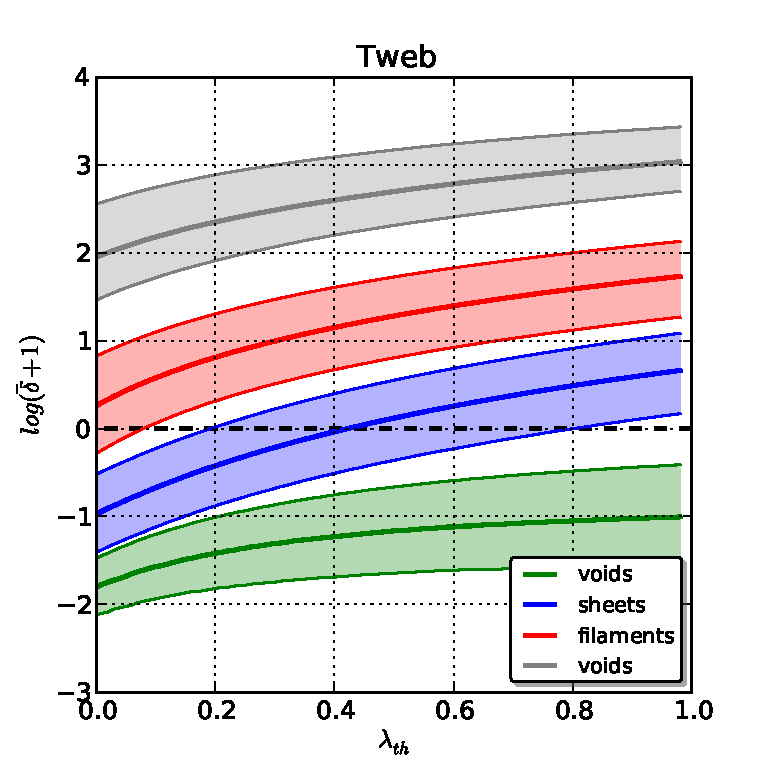
\includegraphics[trim = 0mm 0mm 5mm 5mm, clip, keepaspectratio=true,
  width=0.25\textheight]{./figures/median_environments_densities_Tweb.pdf}
  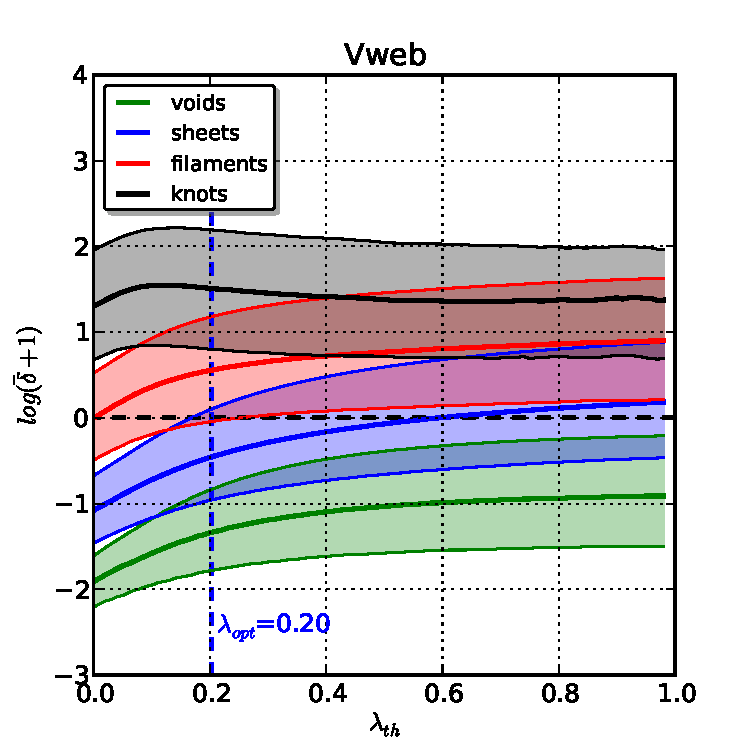
\includegraphics[trim = 0mm 0mm 5mm 5mm, clip, keepaspectratio=true,
  width=0.25\textheight]{./figures/median_environments_densities_Vweb.pdf}
  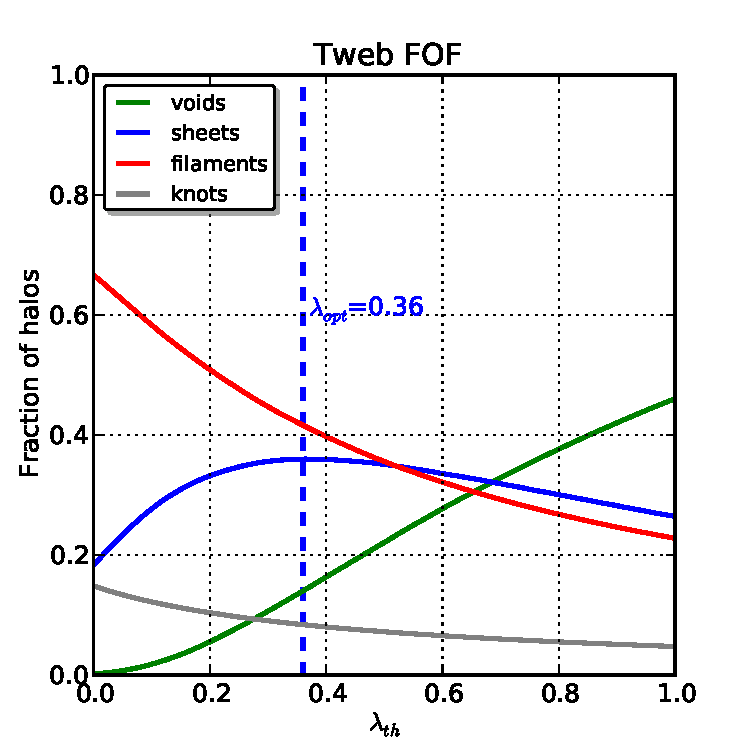
\includegraphics[trim = 0mm 0mm 5mm 5mm, clip, keepaspectratio=true,
  width=0.25\textheight]{./figures/halos_fraction_FOF_Tweb.pdf}
  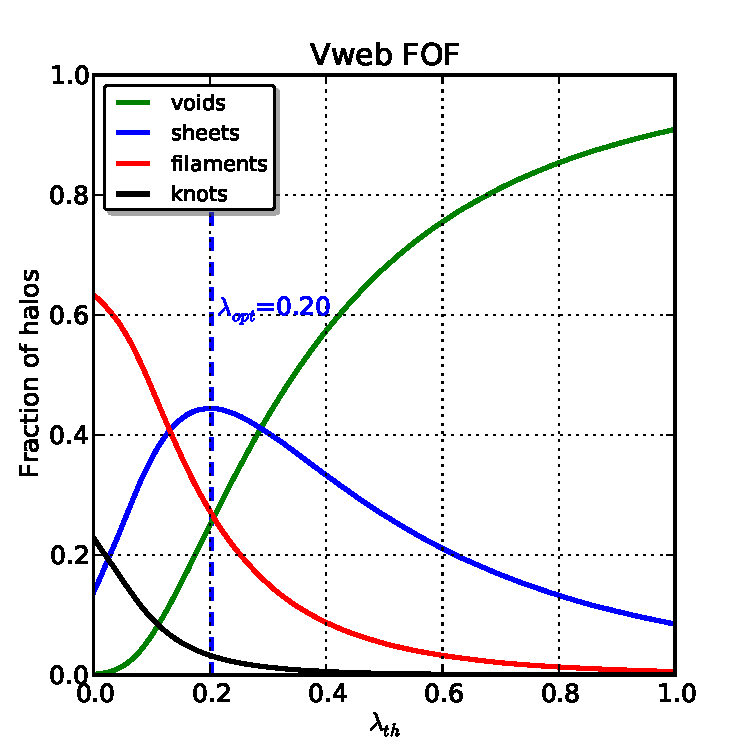
\includegraphics[trim = 0mm 0mm 5mm 5mm, clip, keepaspectratio=true,
  width=0.25\textheight]{./figures/halos_fraction_FOF_Vweb.pdf}

  \captionof{figure}{\small Mean density parameter for each one of the 
  defined environments according to the chosen $\lambda_{th}$ value and 
  for both classification schemes. Tweb (green lines) and Vweb (blue 
  lines). The mean density parameter is calculated by averaging all the 
  values  of the cells determined as a certain type of environment 
  according to its eigenvalues. The optimal parameters found are 
  $\lambda_{opt}^{T}=0.326$ and $\lambda_{opt}^{V}=0.188$.}

  \label{fig:median_density}
  \vspace{0.1 cm}

\end{figure*}
\end{flushleft}
%.........................................................................



%.........................................................................
%FIGURE 2: Visual impresion
\begin{flushleft}
\begin{figure*}
\begin{center}

  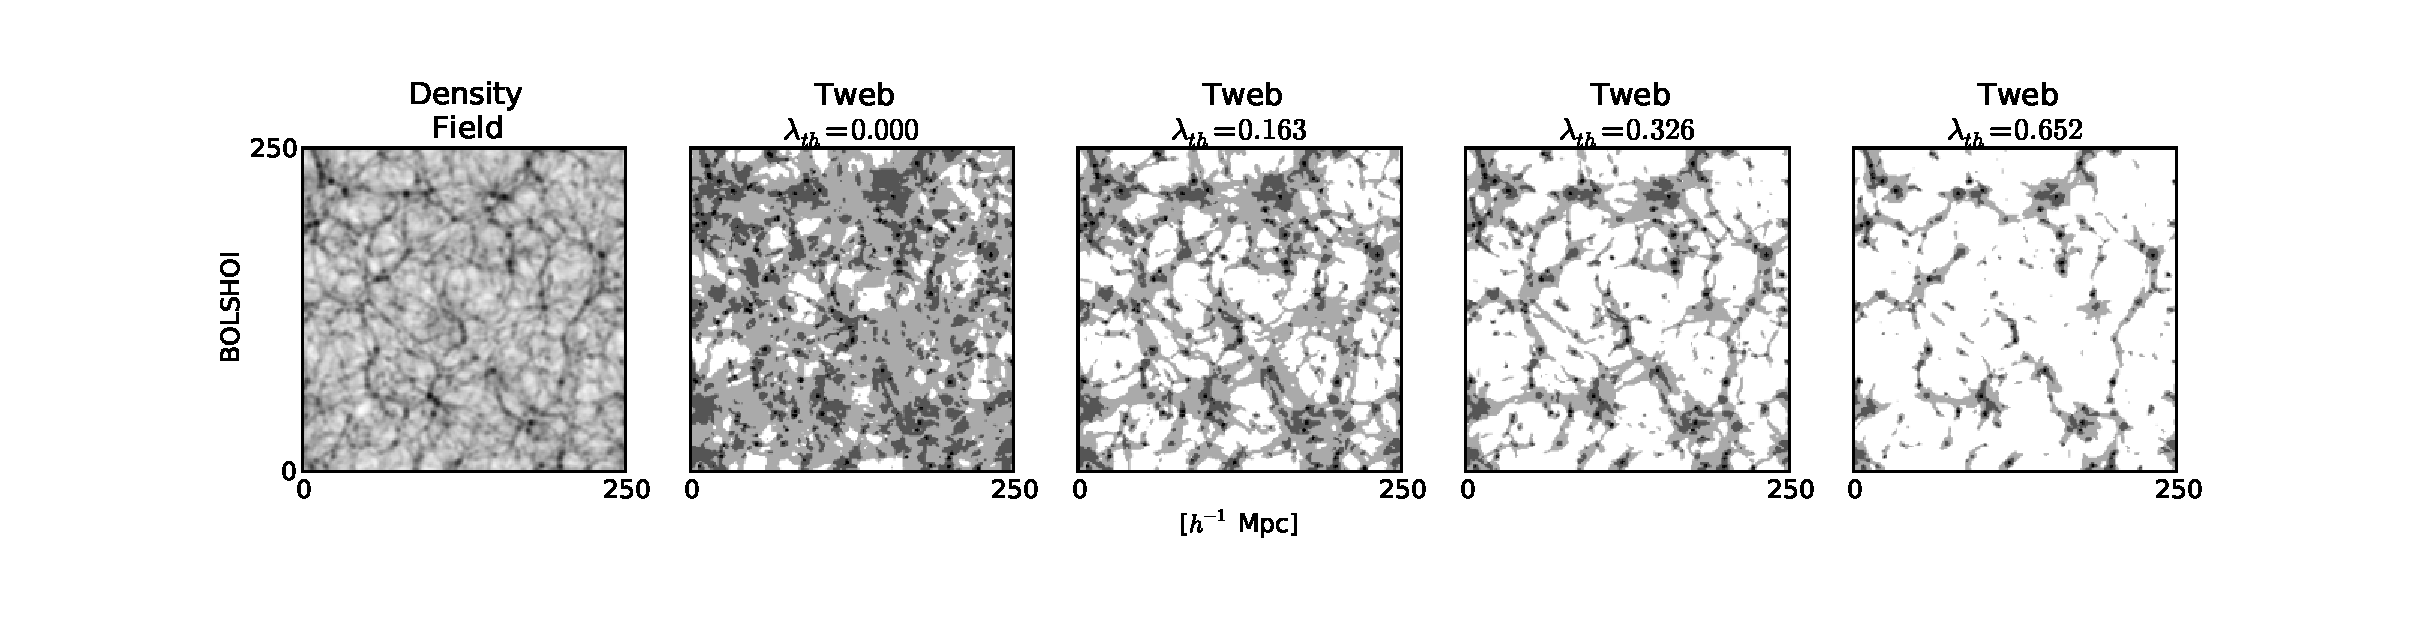
\includegraphics[trim = 42mm 15mm 37mm 10mm, clip, keepaspectratio=true,
  width=0.75\textheight]{./figures/cosmicweb_visual_Tweb.pdf}
  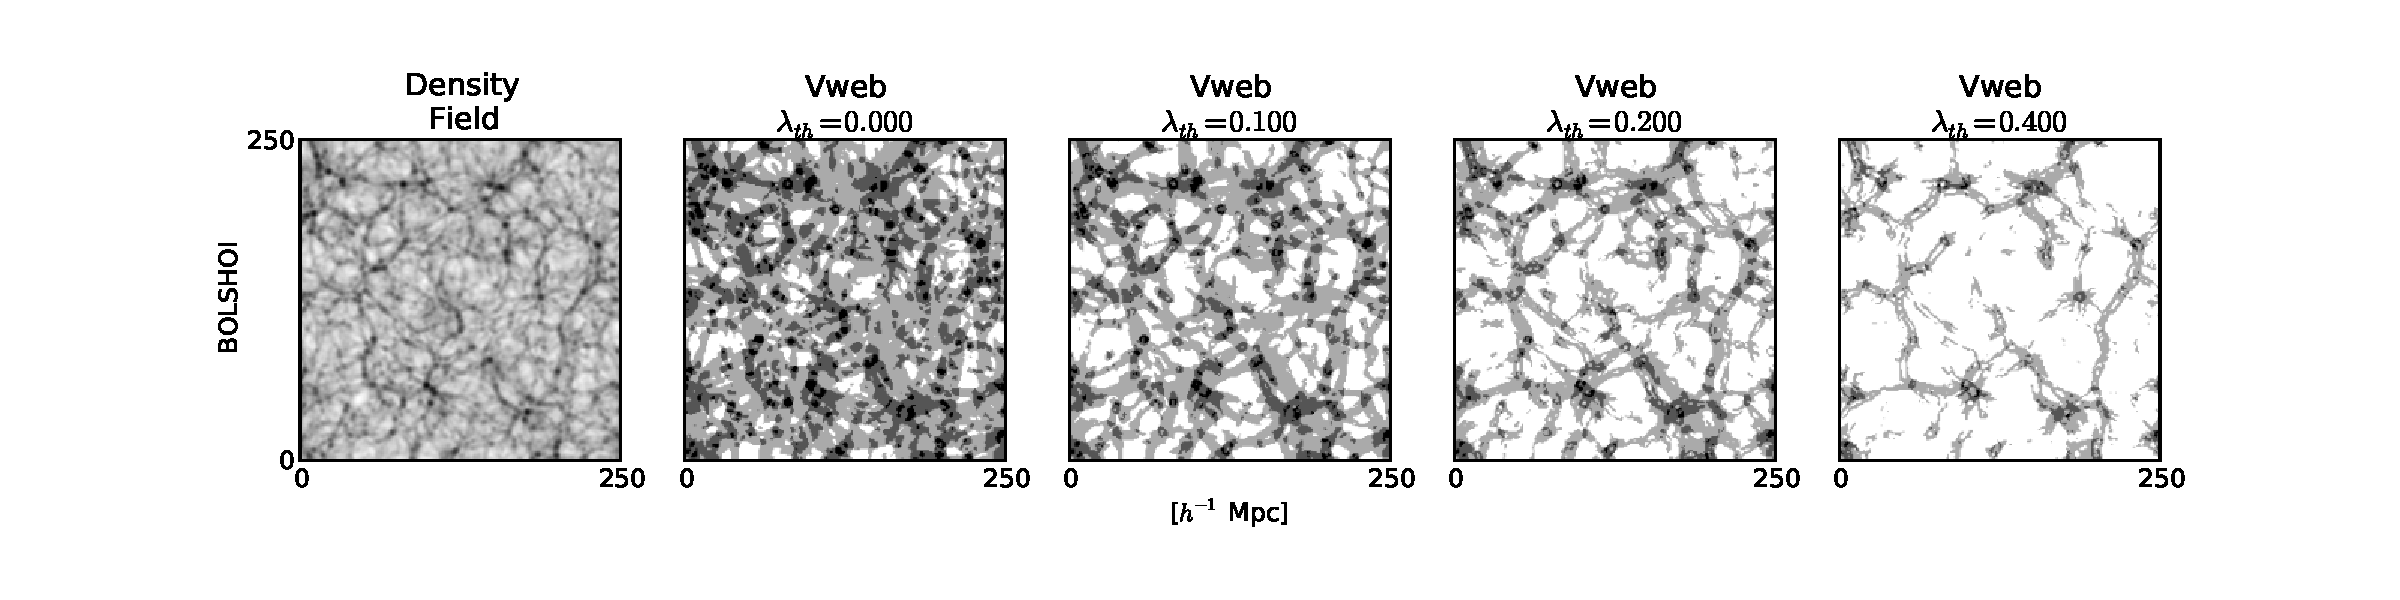
\includegraphics[trim = 42mm 15mm 37mm 10mm, clip, keepaspectratio=true,
  width=0.75\textheight]{./figures/cosmicweb_visual_Vweb.pdf}

  \captionof{figure}{\small Visual impression of the density field (left 
  panels), and of each classification scheme with the $\lambda_{th}$ values 
  obtained by our criteria (others panels). Our color convention for each 
  environment is (white) - void, (light gray) - sheet, (gray) - filament, 
  (black) - knot. For each web scheme, it has been used the previously 
  established optimal threshold as a reference value, so plots are done 
  with the next values $\lambda_{th} = 0.0$, $\lambda_{th} = 
  \lambda_{opt}/2$, $\lambda_{th} = \lambda_{opt}$ and $\lambda_{th} = 
  2\lambda_{opt}$.}

  \label{fig:visual_impression}
  \vspace{0.1 cm}

\end{center}
\end{figure*}
\end{flushleft}
%.........................................................................



%.........................................................................
%FIGURE 3: Percolation analysis
\begin{flushleft}
\begin{figure*}
\begin{center}

  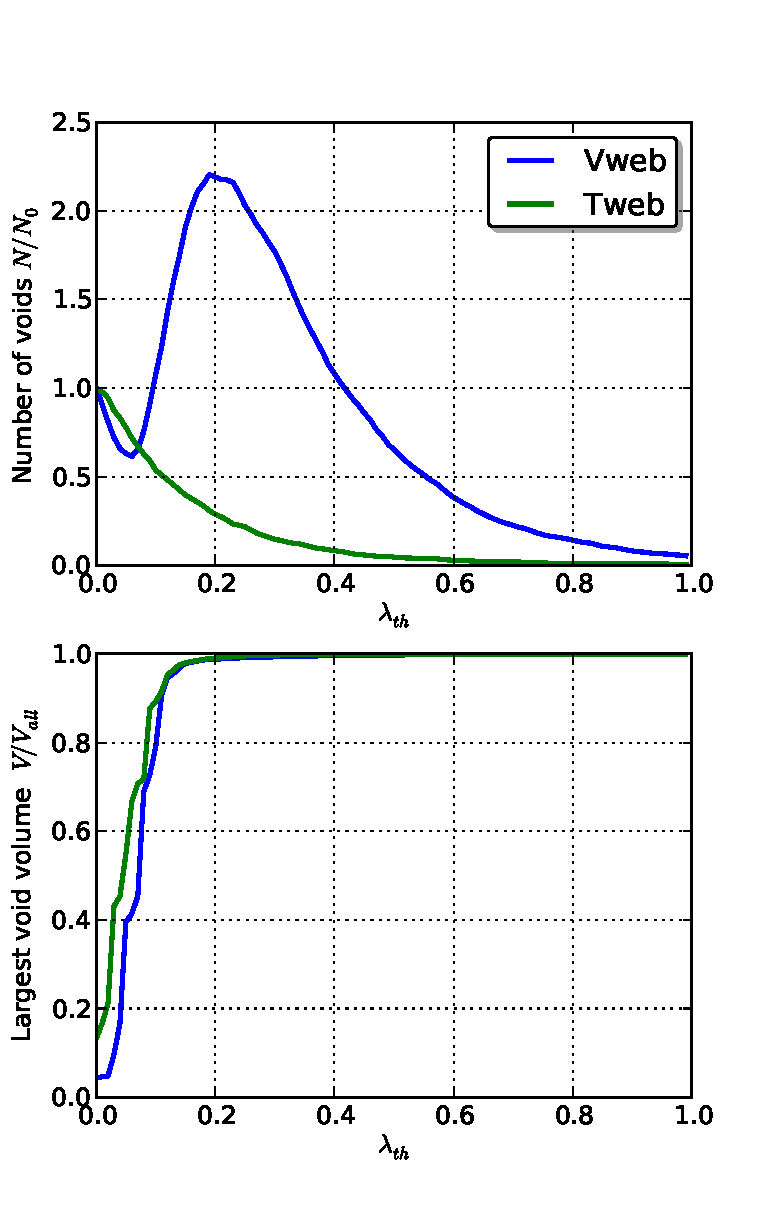
\includegraphics[trim = 1mm 10mm 8mm 18mm, clip, keepaspectratio=true,
  width=0.25\textheight]{./figures/voids_regions_percolation.pdf}
  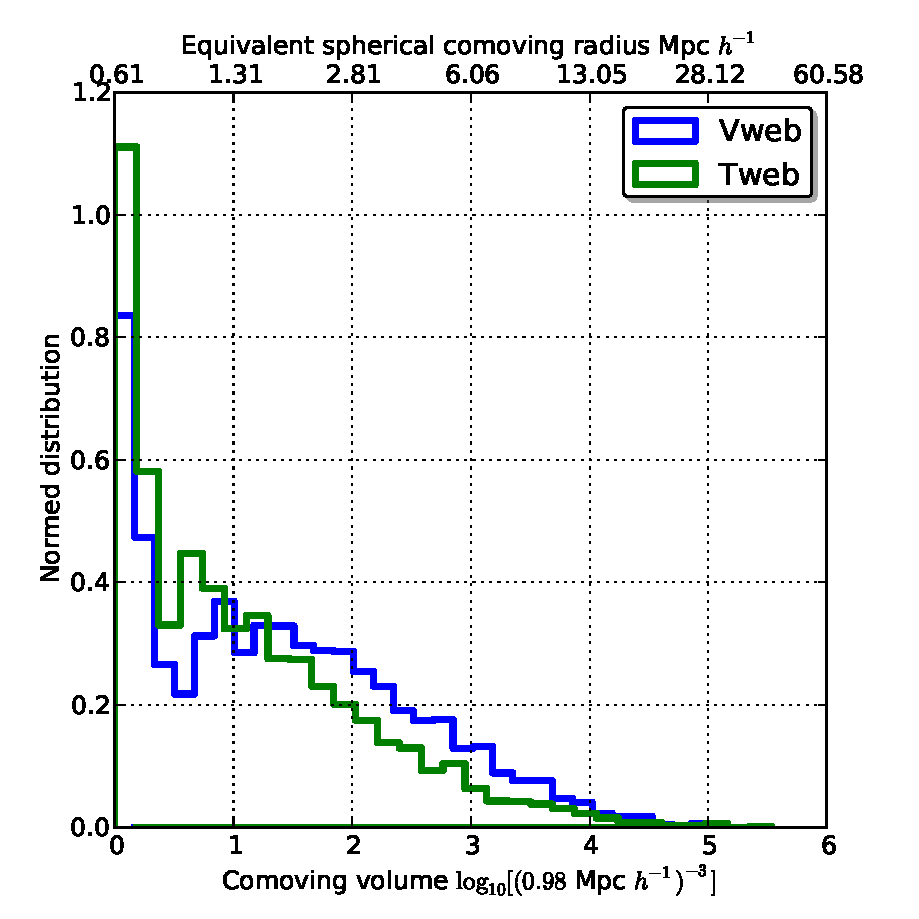
\includegraphics[trim = 0mm 00mm 00mm 00mm, clip, keepaspectratio=true,
  width=0.36\textheight]{./figures/voids_regions_volume.pdf}

  \captionof{figure}{\small Percolation analysis of void regions for 
  different $\lambda_{th}$ values and for both defined classification 
  schemes. T-web (blue lines) and  V-web (green lines). Plot of the largest 
  volume and the number of voids detected according to the threshold value 
  $\lambda_{th}$ (left panels). Size distribution histogram of void cells
  using the threshold value $\lambda_{th} = 0.0$ for both schemes 
  (right panel).}

  \label{fig:percolation_analysis}
  \vspace{0.1 cm}

\end{center}
\end{figure*}
\end{flushleft}
%.........................................................................



%.........................................................................
%FIGURE 4: Distribution of eigenvalues of the inertia tensor
\begin{flushleft}
\begin{figure}
\begin{center}

  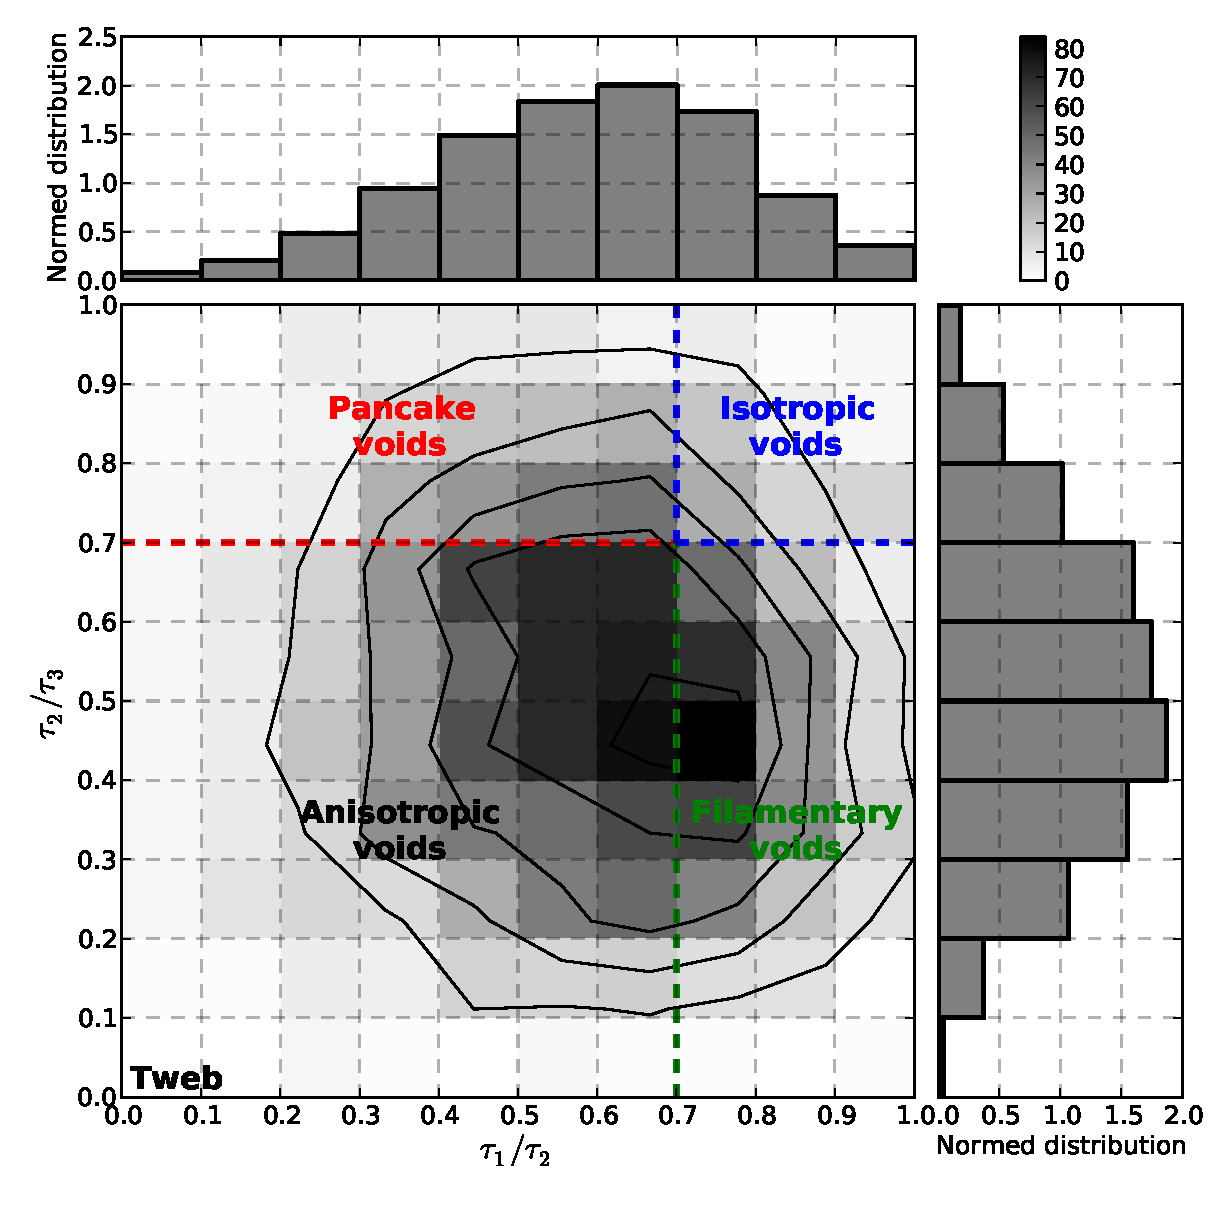
\includegraphics[trim = 7mm 9mm 1mm 0mm, clip, keepaspectratio=true,
  width=0.36\textheight]{./figures/voids_inertia_tensor_Tweb}
  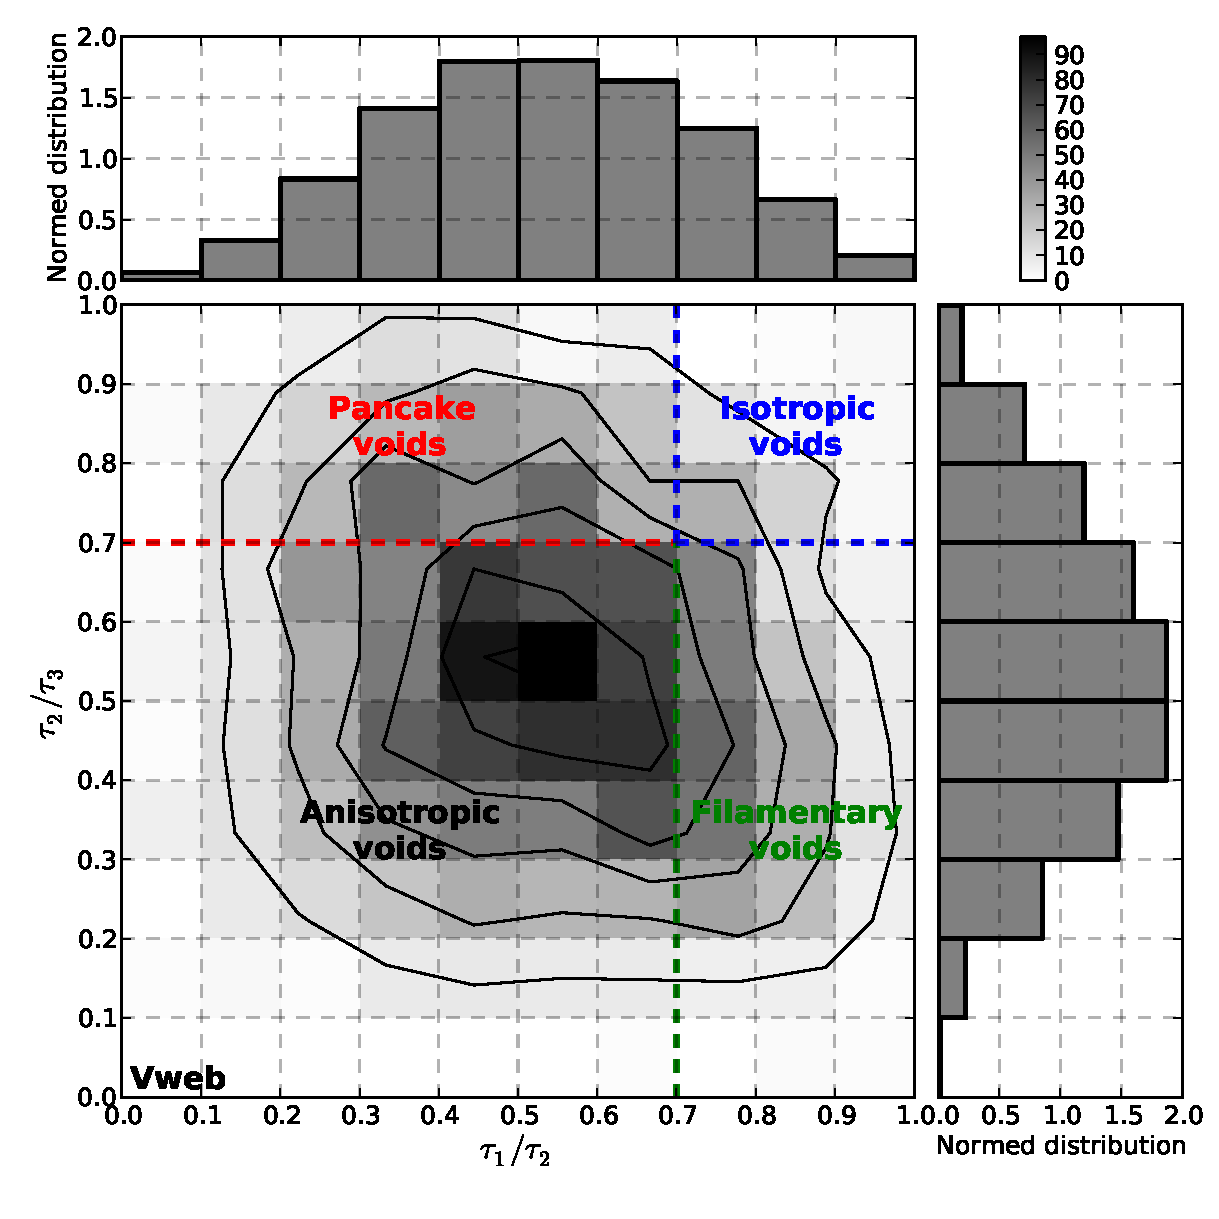
\includegraphics[trim = 7mm 9mm 1mm 0mm, clip, keepaspectratio=true,
  width=0.36\textheight]{./figures/voids_inertia_tensor_Vweb}

  \captionof{figure}{\small Histogram of eigenvalue ratio $\tau_1/\tau_2$
  vs $\tau_2/\tau_3$ for the inertia tensor of void regions. T-web 
  (upper panel) and V-web (lower panel). Number of cells per 
  region in 2D histograms are indicated by the respective colour bar. 
  Upper ($\tau_1/\tau_2$) and right ($\tau_2/\tau_3$) panels of each 
  figure shows a normalized histogram of each ratio parameter. The 
  adopted division for quantify the morphology of void regions is not
  well justified, it should be understood as a fuzzy and continuous 
  limit, done just for illustrative purposes.}

  \label{fig:distro_inertia}
  \vspace{0.1 cm}

\end{center}
\end{figure}
\end{flushleft}
%.........................................................................


%.........................................................................
\end{document}
